\documentclass[pdftex]{beamer}
\usepackage[ruled]{algorithm2e}
\usepackage{algorithmic}
\usepackage{amsmath}
%\usetheme{Frankfurt}

% don't want these in a poster!
\beamertemplatenavigationsymbolsempty

% declare the path(s) where your graphic files are
% ../.. is the GeocronDocuments directory

\graphicspath{{../../images/diagrams/}{../../images/external/location_routing/}}
\DeclareGraphicsExtensions{.pdf,.png}

\begin{document}

\title[Short Title]{Simulating Disaster Scenarios and Geographically-Correlated Resilient Overlay Networks}
\subtitle{Heuristics for Location-based Routing}
\author[K. Benson and Z. Huang]{Kyle E. Benson and Zhipeng Huang}
\institute[UCI]{
  Department of Computer Science\\
  University of California, Irvine\\
  Irvine, California 92697\\[1ex]
  \texttt{kebenson@uci.edu} and \texttt{zhipengh@uci.edu}
}

% % % % % % % % % % % % % % % % % % % % % % % % % % % % % % % % % % % % % % % % % %

\begin{frame}[plain]
	\titlepage
\end{frame}

% % % % % % % % % % % % % % % % % % % % % % % % % % % % % % % % % % % % % % % % % %

\begin{frame}{Challenges}
\begin{columns}
\begin{column}{.5\textwidth}
\begin{itemize}
	\item \textbf{Goal:} Improve data delivery ratio/speed during geographically-correlated network failures
	\item No control over and limited knowledge about routing infrastructure
	\item But can gather location information
	\item \textbf{Claim:} Resilient Overlay Networks can help establish more reliable connections between end-hosts with limited topology knowledge
\end{itemize}
\end{column}

\begin{column}{.5\textwidth}
\begin{figure}
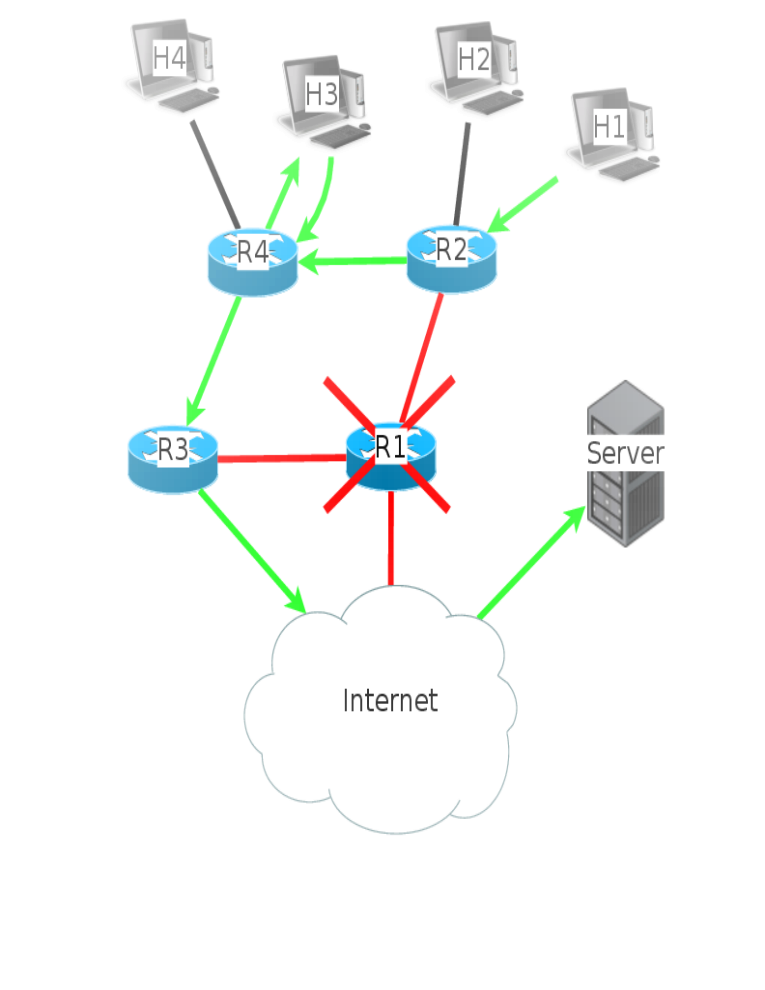
\includegraphics[height=.6\textheight]{overlay_path}
\caption{H1 routes around failed R1 using H3 as an overlay.}
\end{figure}
\end{column}

\end{columns}
\end{frame}

% % % % % % % % % % % % % % % % % % % % % % % % % % % % % % % % % % % % % % % % % %

\begin{frame}{Exploiting Location Information}
\begin{columns}
\begin{column}{.5\textwidth}

\begin{itemize}
	\item Contact overlay nodes outside of local region to avoid failures
	\item Choose overlay nodes from diverse regions not previously attempted
	\item Failure likely along path to server or in local area
	\item Choose node outside local	region to avoid overlapping	paths
	\item Choose path avoiding as much of the direct path as possible
	\item Overlay node may use similar route to sensor
\end{itemize}
\end{column}
	
\begin{column}{.5\textwidth}
\begin{figure}
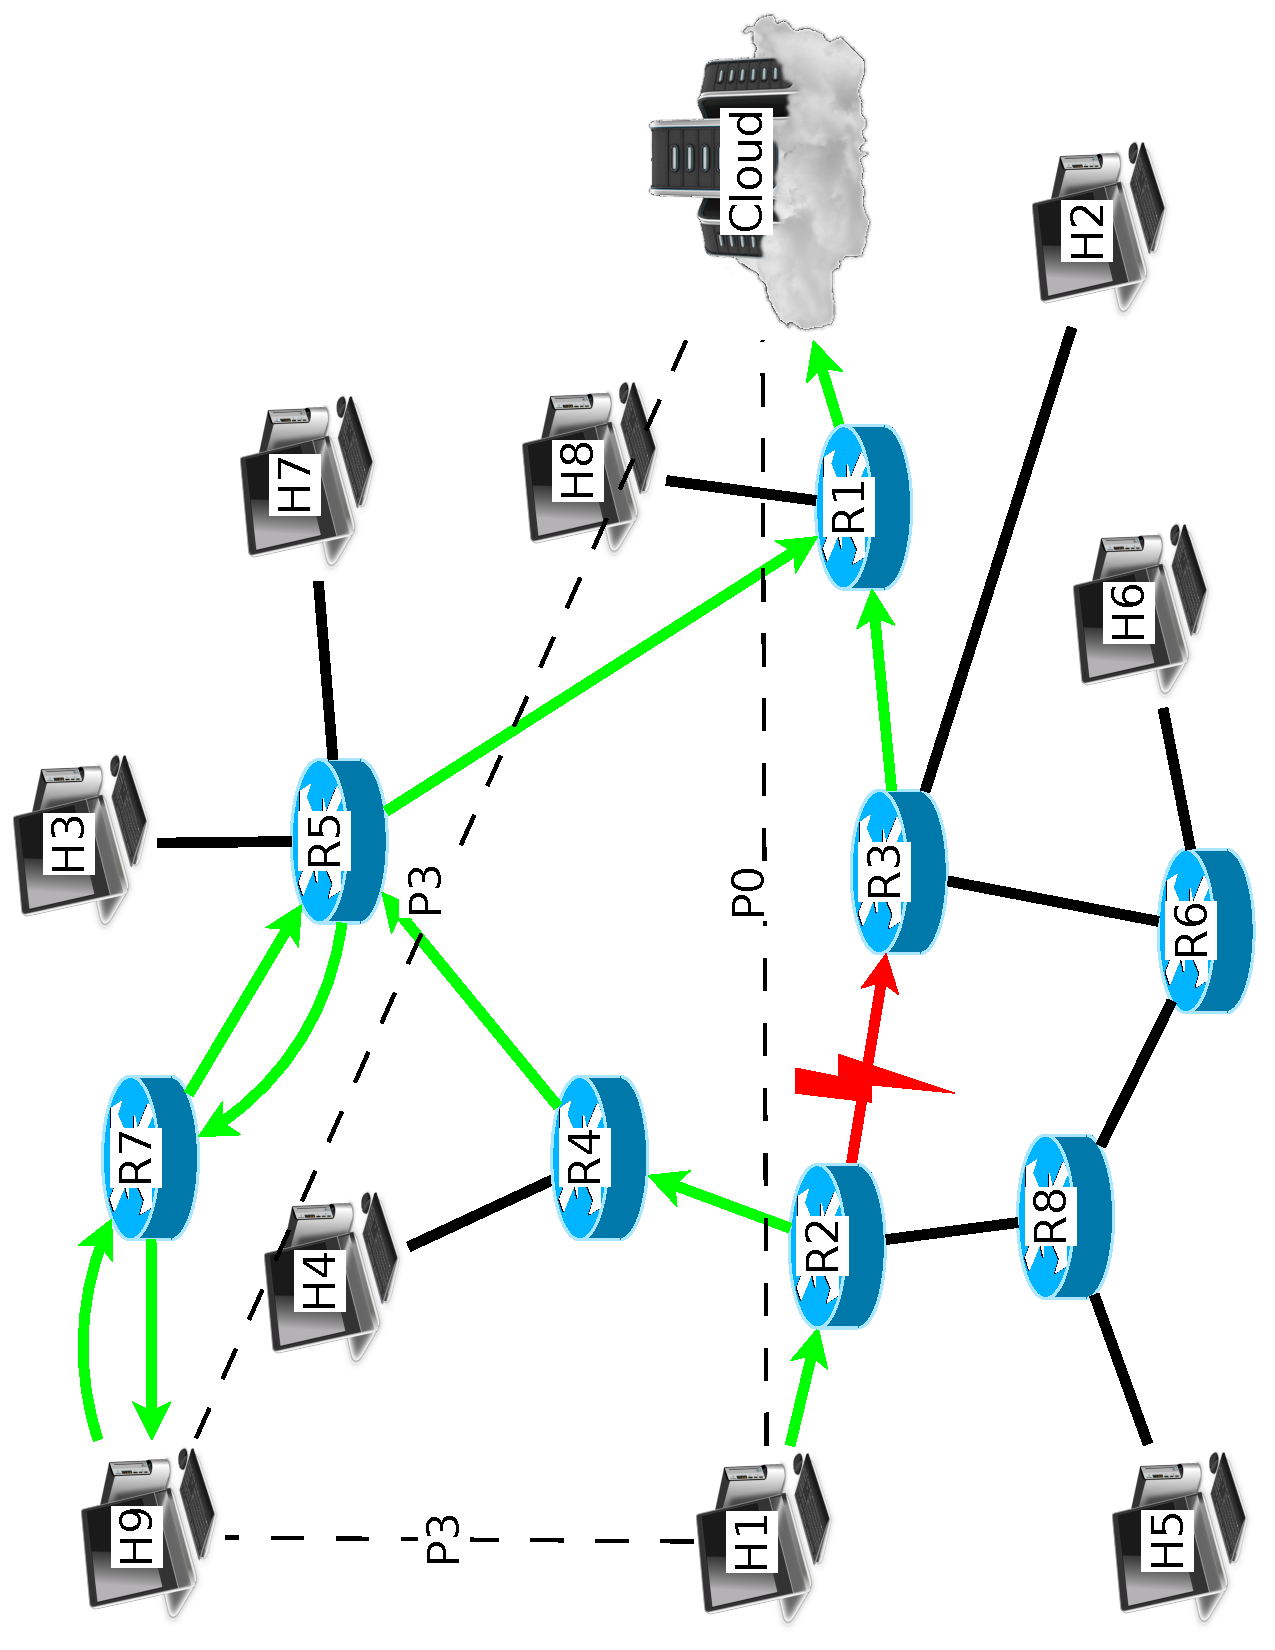
\includegraphics[height=\textwidth,angle=-90]{exploiting_location_information}
\caption{Sensors try to contact nodes outside of the local area and not along the straight-line path to the server.}
\end{figure}
\end{column}

\end{columns}
\end{frame}

% % % % % % % % % % % % % % % % % % % % % % % % % % % % % % % % % % % % % % % % % %

\begin{frame}{Orthogonal Distant Path Heuristic}
\begin{columns}
\begin{column}{.5\textwidth}
\begin{algorithm}[H]
\DontPrintSemicolon
\SetKwBlock{Begin}{begin}{end}
\SetAlgoLined
\SetAlgoLongEnd
\scriptsize
\Begin{
\tcc*[l]{Sensor , overlay and server node are a , b, c respectively}
$idealDist = |0.5 \cdot dist(a,b)|$\;
$perpDist = |\sin (angA) \cdot dist(a,c)|$\;
\lIf{$angA > \frac{\pi}{2}$ {\bf or} $angA + angC < \frac{\pi}{2}$ {\bf or} $perpDist > dist(a,b)$} {$likelihood = 0$\;}
\lElse {$likelihood = 0.5 \cdot (( 1.0 - (||perpDist|-|idealDist|| / idealDist)^{2}) + ( 1.0 - (|\frac{\pi}{2} - angC| / \frac{\pi}{2})^{2}))$\;}
}
\caption{}
\small
\end{algorithm}
\end{column}
	
\begin{column}{.5\textwidth}
\begin{figure}
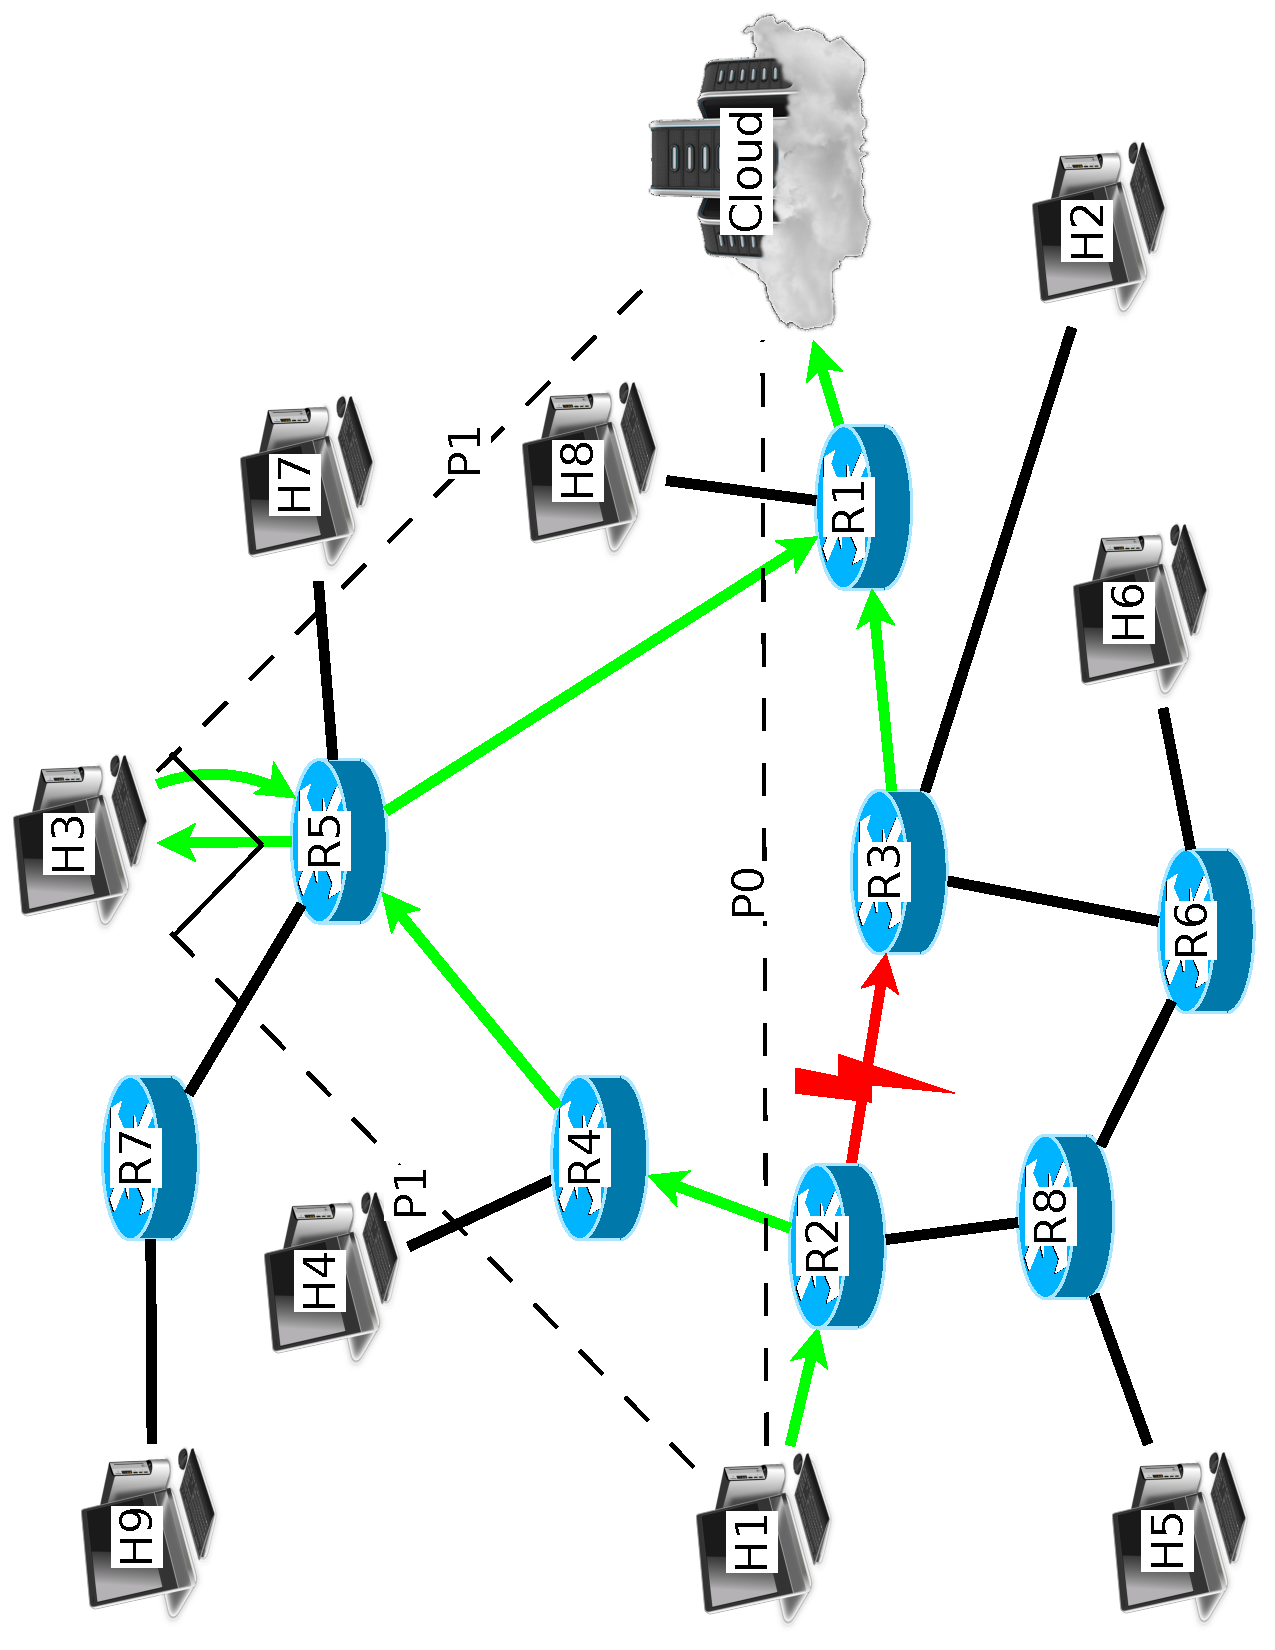
\includegraphics[height=\textwidth,angle=-90]{angular_path}
\caption{The intuition of this heuristic is to avoid the straight path, without diverging from it too much.  It strikes a middle ground by choosing a path at an ideal angle of $45^{\circ}$, which makes the angle at the top orthogonal, hence the name.}
\end{figure}
\end{column}

\end{columns}
\end{frame}

% % % % % % % % % % % % % % % % % % % % % % % % % % % % % % % % % % % % % % % % % %

\begin{frame}{New Region Heuristic}
\begin{columns}
\begin{column}{.5\textwidth}
\begin{algorithm}[H]
\DontPrintSemicolon
\SetKwBlock{Begin}{begin}{end}
\SetAlgoLined
\SetAlgoLongEnd
\scriptsize
\Begin{
%\tcc*[l]{Discover any node that has not been discoverd in this region}
\lIf{$RegionsAttempCount (RegionCount)$} {$likelihood = 0$\;}
\lElse {$likelihood = 1.0$\;}
}
\caption{}
\small
\end{algorithm}
\end{column}
	
\begin{column}{.5\textwidth}
\begin{figure}
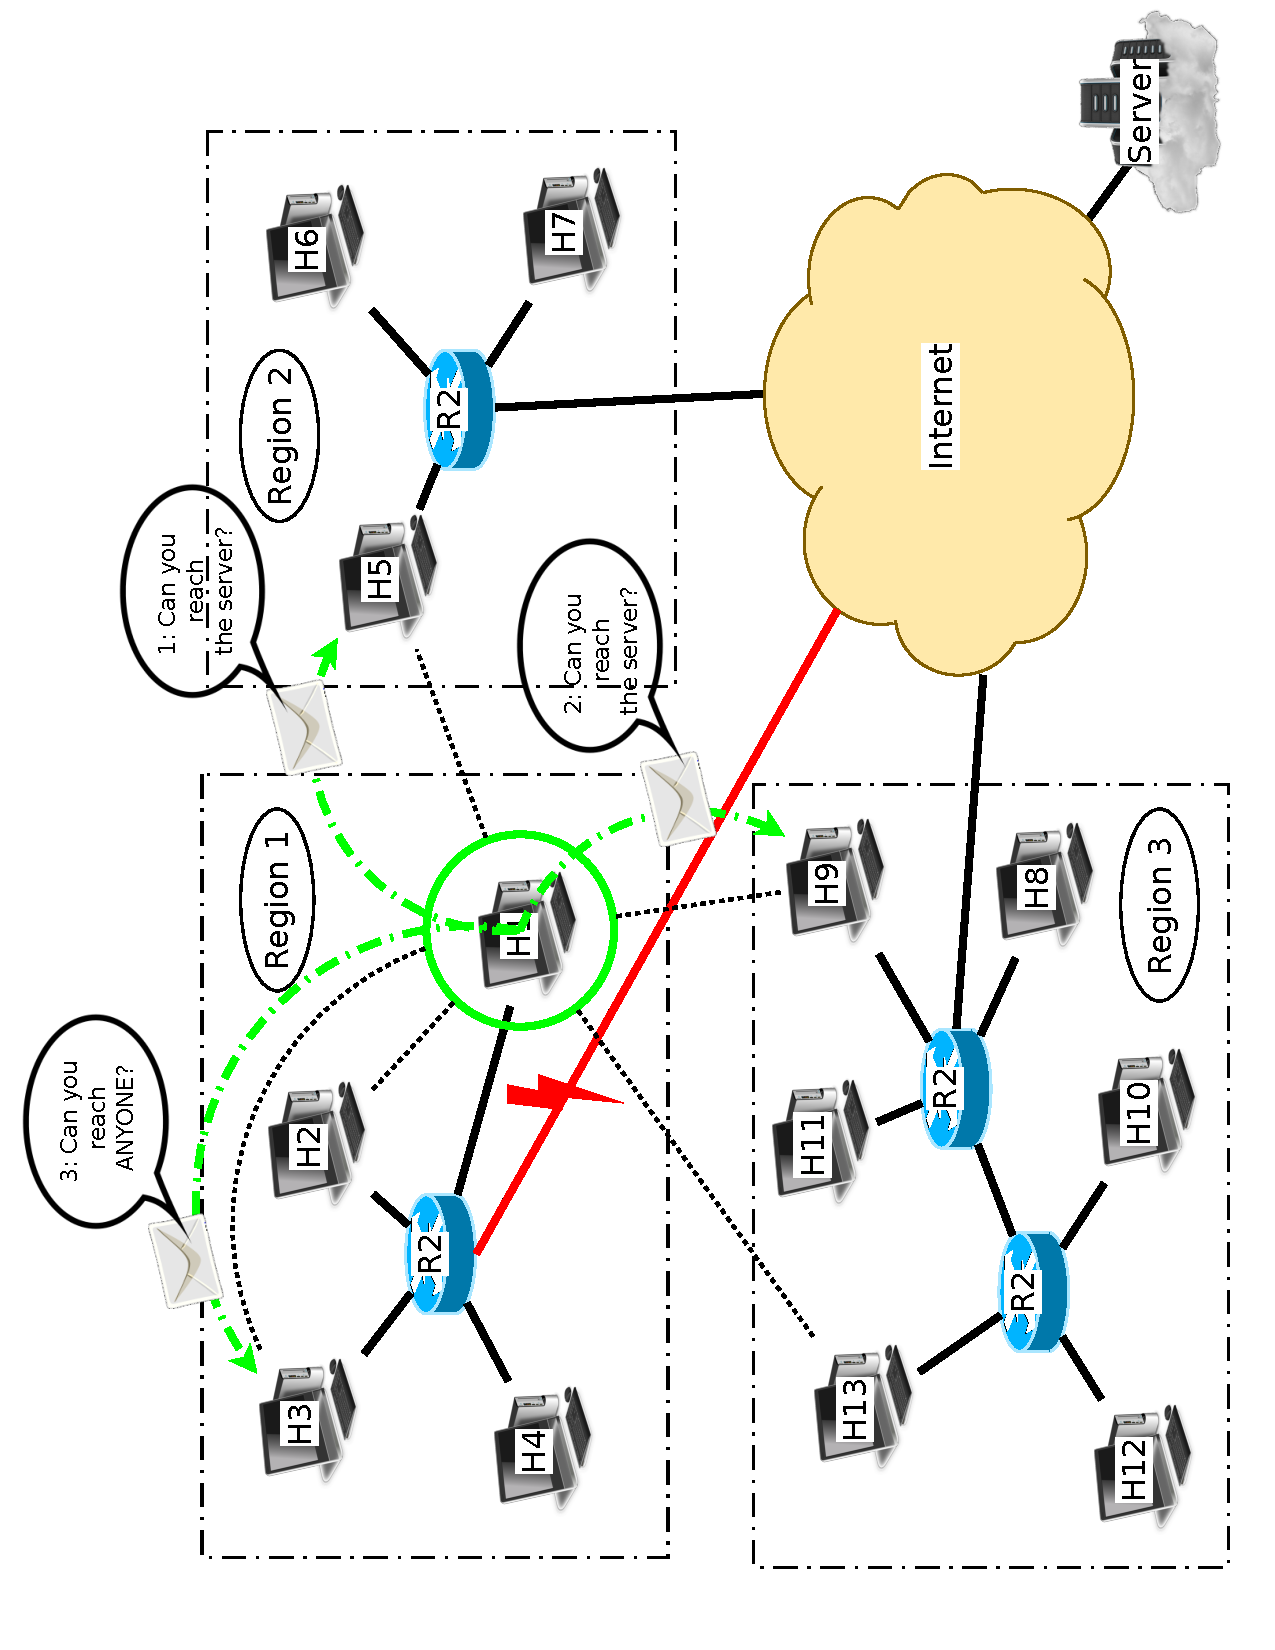
\includegraphics[height=\textwidth,angle=-90]{new_region_all}
\caption{The intuition of this heuristic is to avoid regions that have been previously attempted unsuccessfully.  We assume that no further attempts to contact such a region will succeed.}
\end{figure}
\end{column}

\end{columns}
\end{frame}

% % % % % % % % % % % % % % % % % % % % % % % % % % % % % % % % % % % % % % % % % %
\begin{frame}{New Angle Path Heuristic}
\begin{columns}

\begin{column}{.5\textwidth}
\begin{algorithm}[H]
\DontPrintSemicolon
\SetKwBlock{Begin}{begin}{end}
\SetAlgoLined
\SetAlgoLongEnd
\scriptsize
\Begin{
%\tcc*[l]{The angle could be either acute or obtuse.}
$angle = AngleBetween ((sensor,overlay),(sensor,server))$
\lFor {$(path = pathsAttempted)$\;}
\lIf{$angle = \pi$ {\bf or} $angle = 0$} {$likelihood = 0$\;}
\lElseIf{$angle < \pi$} {$likelihood = \cos (angle - \frac{\pi}{4})$\;}
\lElseIf{$angle > \pi$} {$likelihood = \cos (2 \cdot ((2\pi - angle) - \frac{\pi}{4})/3)$\;}
$likelihood = likelihood \cdot pastLikelihood$\;
%\tcc*[l]{aggregate likelihoods to make punishments on wrong choices}
}
\caption{}
\small
\end{algorithm}
\end{column}
	
\begin{column}{.5\textwidth}
\begin{figure}
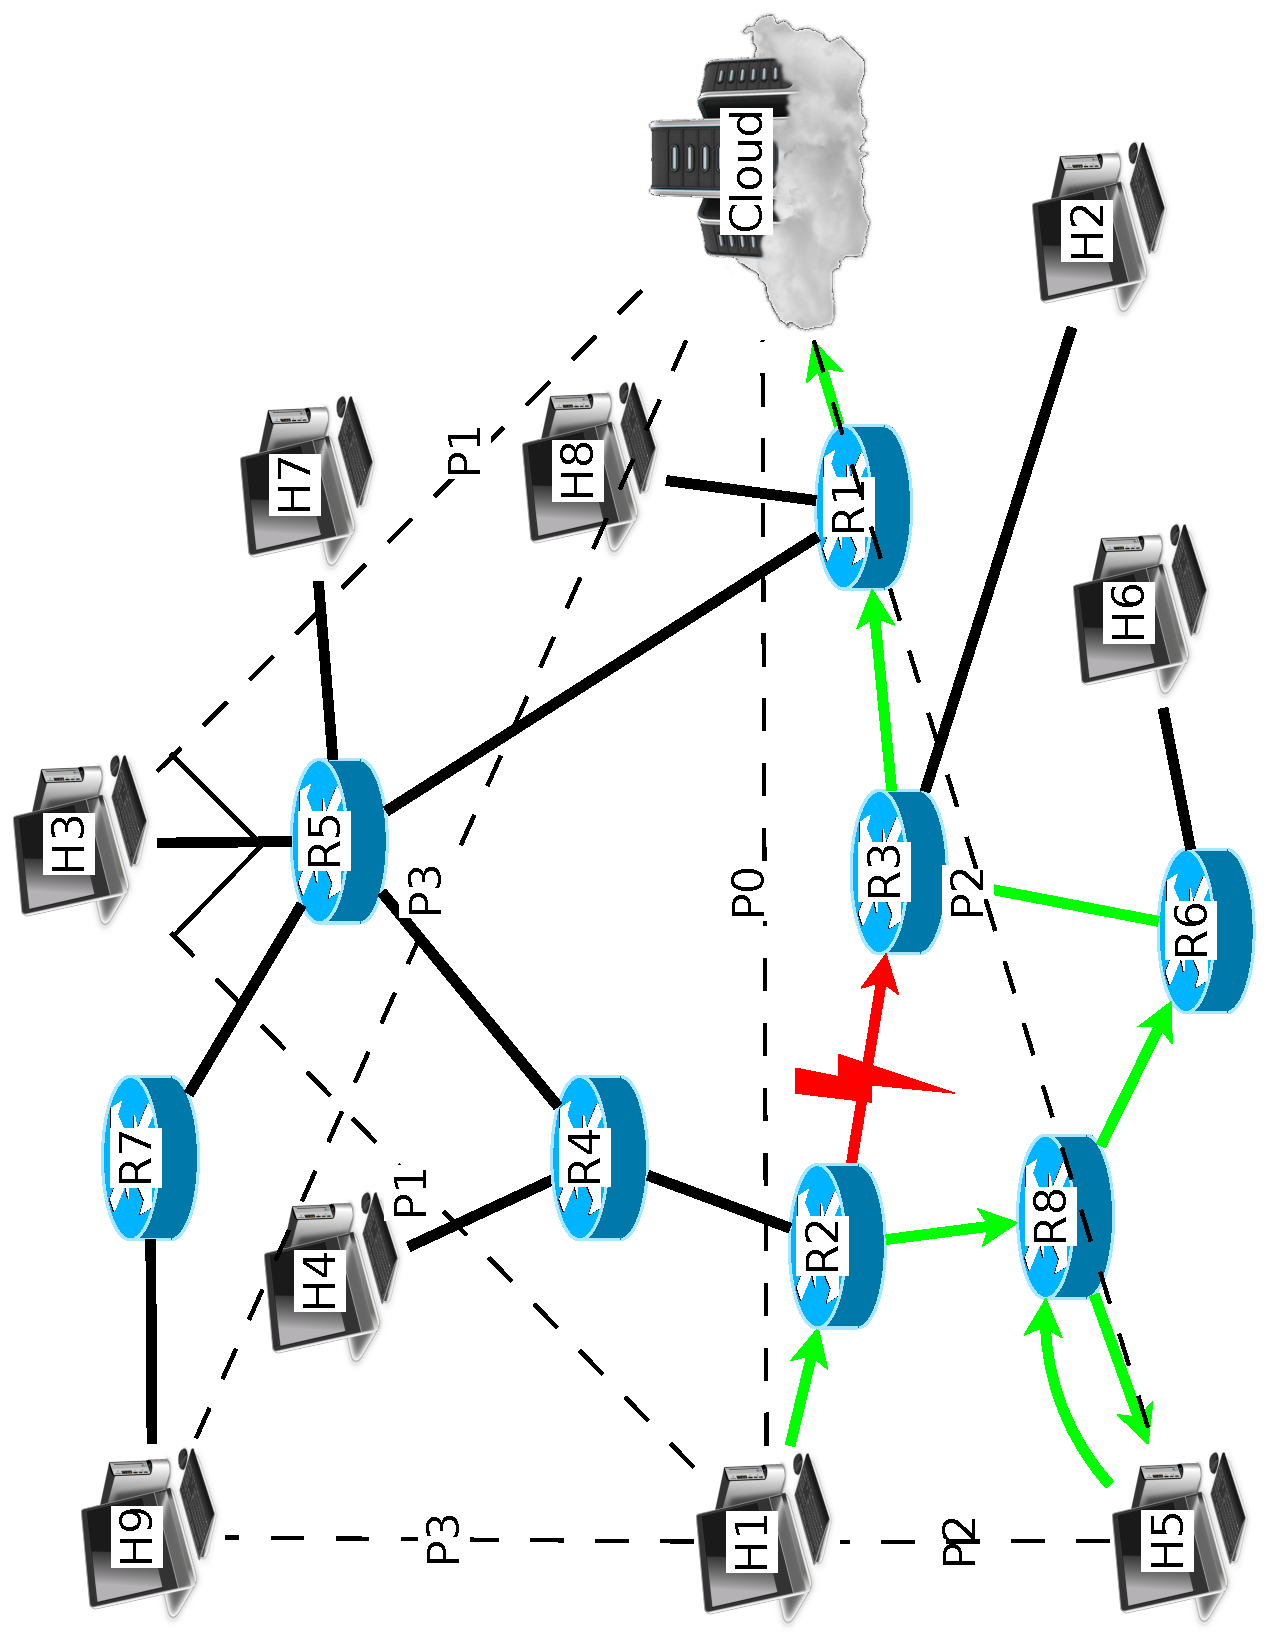
\includegraphics[height=\textwidth,angle=-90]{new_angle}
\caption{This heuristic attempts paths along new angles different from the ones previously attempted.}
\end{figure}
\end{column}

\end{columns}
\end{frame}

% % % % % % % % % % % % % % % % % % % % % % % % % % % % % % % % % % % % % % % % % %

\begin{frame}{Distance-Dependent Path Heuristic}
\begin{columns}
\begin{column}{.5\textwidth}

\begin{algorithm}[H]
\DontPrintSemicolon
\SetKwBlock{Begin}{begin}{end}
\SetAlgoLined
\SetAlgoLongEnd
\scriptsize
%\SetAlgoSkip{bigskip}
%\SetAlgoInsideSkip{medskip}
%$/*Initialization*/$\;
\Begin{
%\tcc*[l]{Define idealDist as half of the distance from the source to the destination, dist as the distance from the source to the candidate node, minDist as a lower boundary to avoid candidate node being too close to the source.}
$idealDist = 0.5 * dist(sensor,server)$
$minDist = certain reasonably small number$
$dist = dist(sensor,overlay)$
\lIf{$dist <= minDist$} {$likelihood = 0$\;}
\lElseIf{$minDist < dist < idealDist$} {$likelihood = dist^{2} / idealDist^{2}$\;}
\lElseIf{$dist >= idealDist$} {$likelihood = idealDist / dist $\;}
}
\caption{}
\small
\end{algorithm}
\end{column}
	
\begin{column}{.5\textwidth}
\begin{figure}
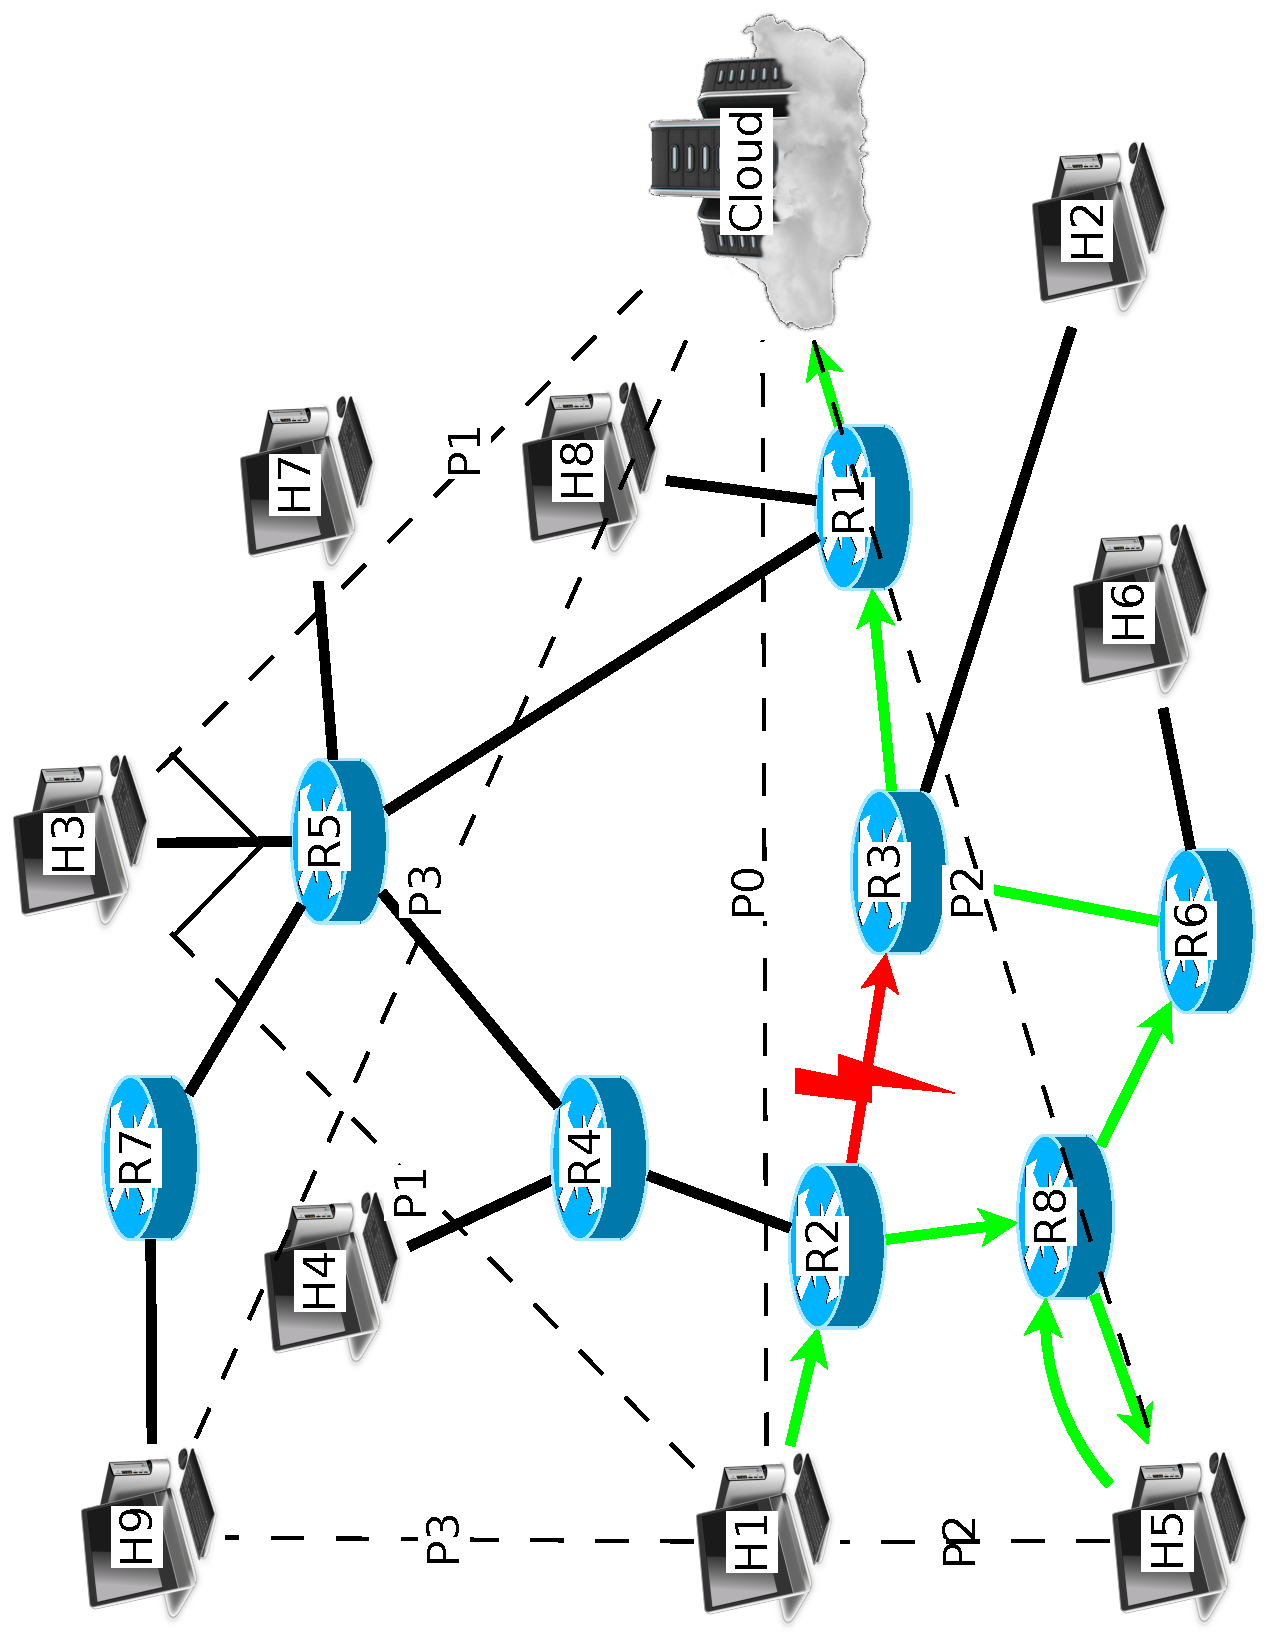
\includegraphics[height=\textwidth,angle=-90]{new_angle}
\caption{This heuristic attempts paths that use overlay nodes at an ideal distance from the sensor.  This ideal distance is chosen as a radius that reaches half-way to the server.}
\end{figure}
\end{column}

\end{columns}
\end{frame}

% % % % % % % % % % % % % % % % % % % % % % % % % % % % % % % % % % % % % % % % % %

\begin{frame}{Furthest First Path Heuristic}
\begin{columns}
\begin{column}{.5\textwidth}
\begin{figure}
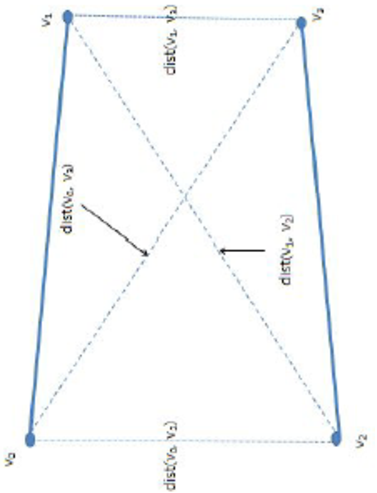
\includegraphics[height=.6\textwidth,angle=-90]{path_similarity_two_destinations}
\caption{Definition of path similarity presented in W. Sun, ``A Method for Overlay Network Latency Estimation from Previous Observation'', ICN-2013.}
\end{figure}

\Tiny{

$geo\_similarity(v_0, v_1, v_2, v_3) = $\\
$\min[dist(v_0, v_2) + dist(v_1, v_3), dist(v_0, v_3) + dist(v_1, v_2)]$

}

\vspace{8pt}
When considering one server,
\vspace{8pt}

\Tiny{
$geo\_similarity(v_0, v_1, v_2, v_3) = $\\
$dist(v_0, v_2) = geo(v_0, v_2)$
}
\end{column}
	
\begin{column}{.5\textwidth}
\begin{figure}
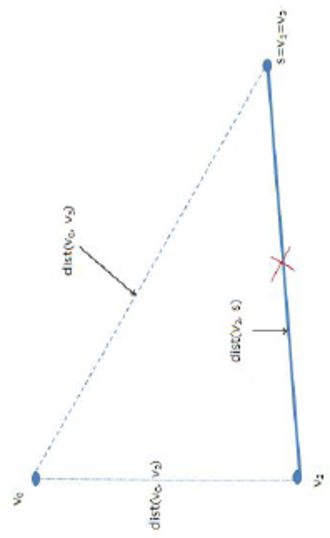
\includegraphics[height=.6\textwidth,angle=-90]{path_similarity_one_destination}
\caption{Thus, this heuristic considers overlay peers located further away to be more likely candidates.}
\end{figure}

\begin{algorithm}[H]
\DontPrintSemicolon
\SetKwBlock{Begin}{begin}{end}
\SetAlgoLined
\SetAlgoLongEnd
\scriptsize
\Begin{
\tcc*[l]{maxDistance = certainly reasonably large number}
\lIf{$dist(a,b) > maxDistance$} {$likelihood = 0$\;}
\lElse {$likelihood = (maxDistance - dist(a,b)) / maxDistance $\;}
}
\small
\end{algorithm}
\end{column}

\end{columns}
\end{frame}

% % % % % % % % % % % % % % % % % % % % % % % % % % % % % % % % % % % % % % % % % %

\begin{frame}{Closest First Path Heuristic}
\begin{columns}
\begin{column}{.5\textwidth}
\begin{algorithm}[H]
\DontPrintSemicolon
\SetKwBlock{Begin}{begin}{end}
\SetAlgoLined
\SetAlgoLongEnd
\scriptsize
\Begin{
\tcc*[l]{minDistance = certain reasonably small number}
\lIf{$dist(a,b) < minDistance$} {$likelihood = 0$\;}
\lElse {$likelihood = (dist(a,b) - minDistance) / dist(a,b) $\;}
}
\caption{}
\small
\end{algorithm}
\end{column}
	
\begin{column}{.5\textwidth}
\begin{figure}
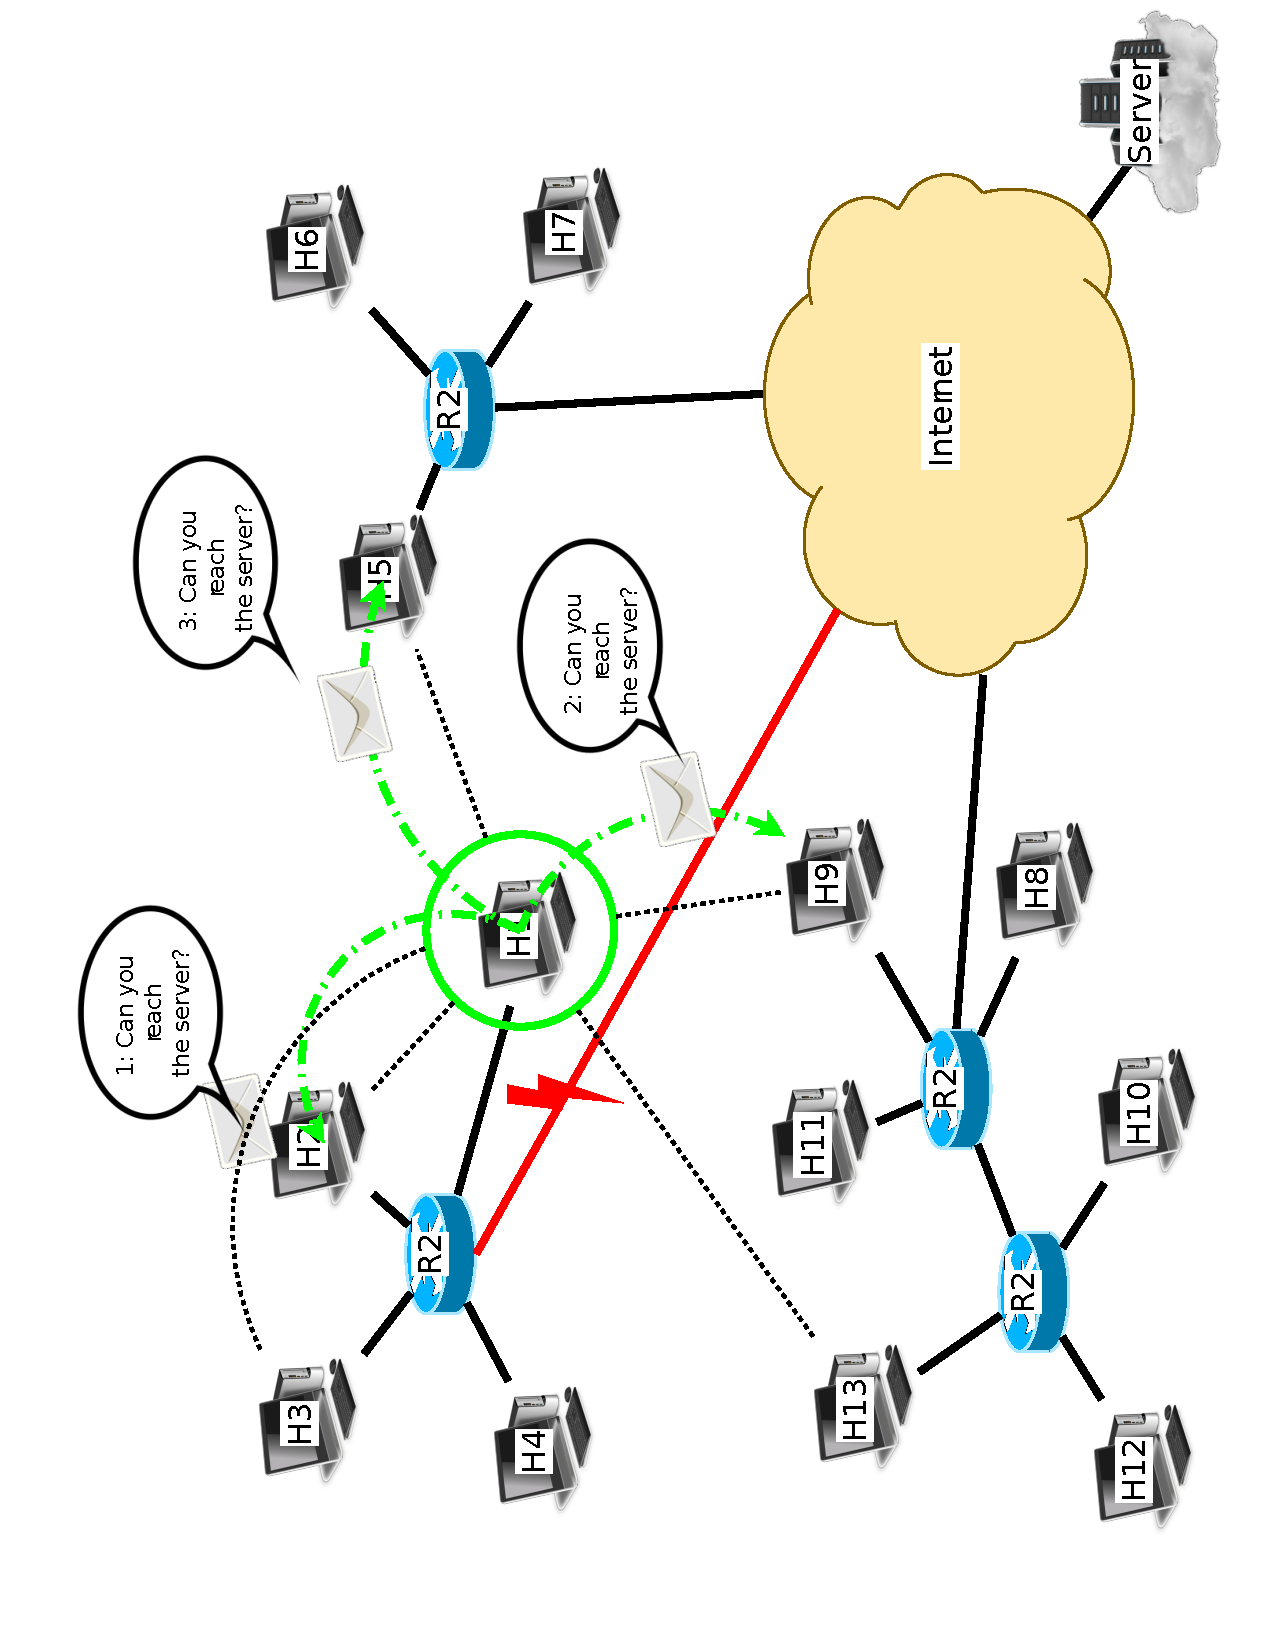
\includegraphics[height=\textwidth,angle=-90]{nearest_neighbor}
\caption{The intuition of this heuristic is to contact nearby overlay nodes that have found a path out of the local region.  We found, however, that this approach does not always work well in practice, likely due to the path similarity inherent with nearby nodes.}
\end{figure}
\end{column}

\end{columns}
\end{frame}


% % % % % % % % % % % % % % % % % % % % % % % % % % % % % % % % % % % % % % % % % %

%\begin{frame}{Regions/AS'es Evaluated}
%\begin{columns}
%\begin{column}{\textwidth}
%\begin{table}
%\centering
%\label{TABLE}
%\caption{}
%\begin{tabular}{|c|c|c|c|c|l|l|l|l|l|l|l|l|}
%  \hline
%  % after \\: \hline or \cline{col1-col2} \cline{col3-col4} ...
%   &  &  &  &  &  &  &  \\
%  \hline
%  Disaster Region         &  &  &  &  &  &  &  \\
%  \hline
%  Total Nodes             &  &  &  &  &  &  &  \\
%  \hline
%  Total Overlay Nodes     &  &  &  &  &  &  &  \\
%  \hline
%  Nodes in Region         &  &  &  &  &  &  &  \\
%  \hline
%  Overlay Nodes in Region &  &  &  &  &  &  &  \\
%  \hline
%\end{tabular}
%\end{table}
%\end{column}
%\end{columns}
%\end{frame}

% % % % % % % % % % % % % % % % % % % % % % % % % % % % % % % % % % % % % % % % % %

\begin{frame}{Furthest First Path Heuristic}
\begin{itemize}
	\item Compared heuristics with baseline Random
	\item ns-3 simulation environment
	\item 10 seconds simulation time
	\begin{itemize}
		\item $>$10s $\rightarrow$ data not as useful for early warning
		\item Most damage done (earthquake over)
		\item Routes start to recover
	\end{itemize}
	\item Nodes retry every $timeout$ seconds (up to 20 times)
	\item $timeout = 500ms$: East $\rightarrow$ West RTT $\approx$200-300ms
	\item Nodes/links in disaster region fail uniformly with probability $p = 0.1, 0.2, 0.3, 0.4, 0.5$
	\item All overlay nodes in region (one incident link) report to server during disaster
	\item Server chosen randomly from 10 highest-degree nodes outside disaster
	\item Each combination of parameters repeated 100 times with different RNG seeds
	\item BRITE topology generator (10,000 nodes, 50 AS'es, top-down Barabasi/Waxman model, 25 regions)
\end{itemize}
\end{frame}

% % % % % % % % % % % % % % % % % % % % % % % % % % % % % % % % % % % % % % % % % %

%
%\part{rest}
%
%\begin{frame}{Roadmap}
%	\tableofcontents
%\end{frame}
%
%\section{Location Service}
%
%\begin{frame}{Location Service}
%\begin{columns}
%\begin{column}{.5\textwidth}
%
%	\begin{itemize}
%		\item Nodes have GPS
%		\item But how to look up destination's location?
%		\item Maintain global information \uncover<2->{\alert{easily outdated/inefficient}}
%		\item<3-> Distribute load
%		\begin{itemize}
%			\item In , node updates \emph{location servers} (LS) throughout network
%			\item Divide network into hierarchical grid
%			\item LS's in 3 external grids at each level
%			\item Lookup distance $<$ square LS co-resides in
%		\end{itemize}
%		
%	\end{itemize}
%
%\end{column}
%
%\begin{column}{.5\textwidth}
%\uncover<3->{
%\begin{figure}
%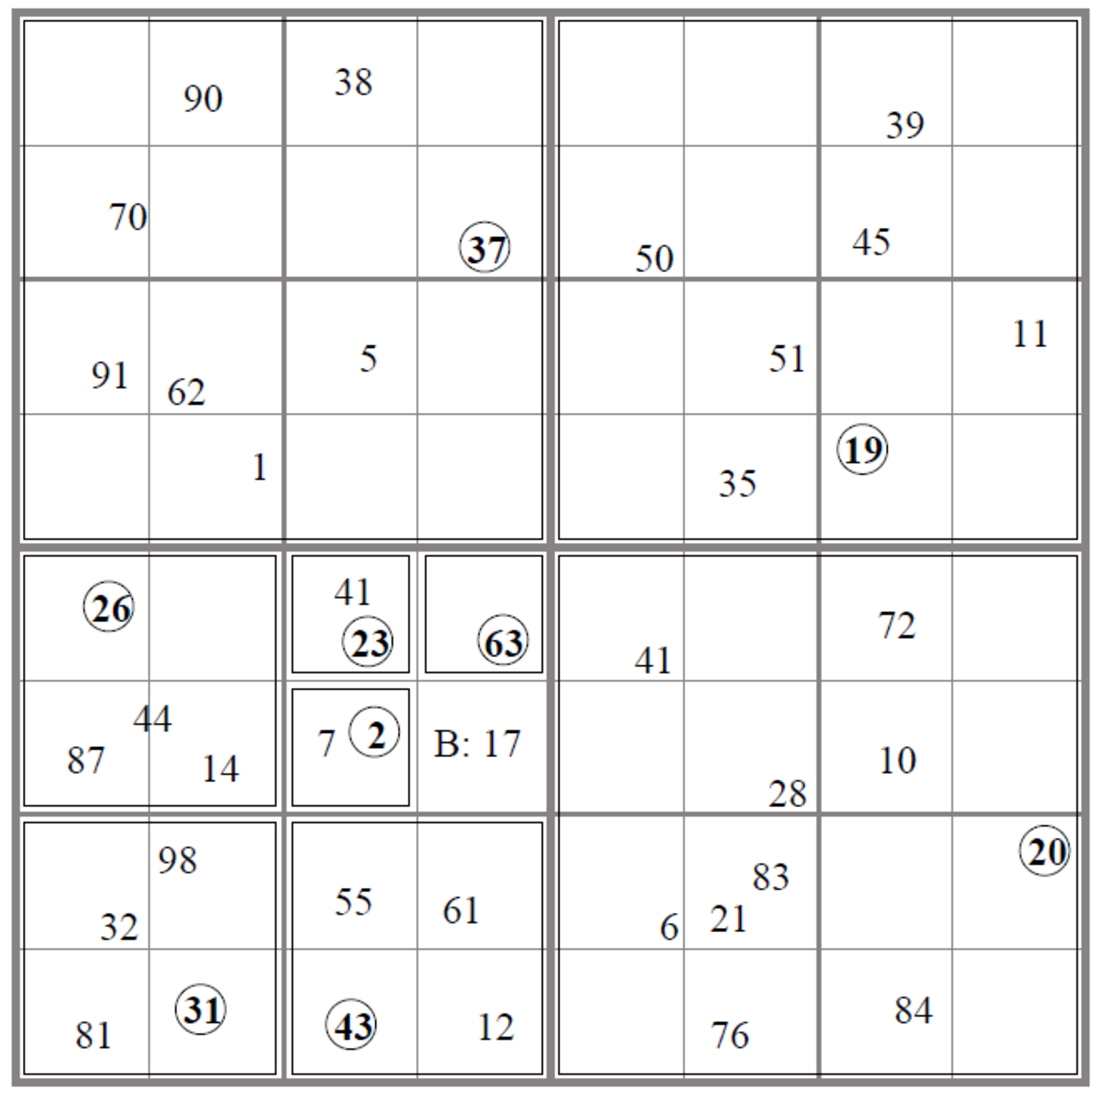
\includegraphics[width=\textwidth]{location_service}
%\caption{Hierarchical grid with 4 order-i squares in order-i+1 square.}
%\end{figure}}
%\end{column}
%\end{columns}
%\end{frame}
%

\end{document}
